\documentclass[12pt,letterpaper]{article}
\usepackage{apa_manual}
\apatituloCorto{Reservorios clásicos ESN y cuánticos QRC}

\begin{document}

\apacabecera
  {Redes de Reservorio (ESN), Características Aleatorias (RFF) y Reservorios Cuánticos (QRC)}
  {Manual teórico y práctico 6 — Fundamento y resultados de la Etapa 4}
  {Con apenas \(90\) a \(339\) observaciones mensuales disponibles en cada ventana de entrenamiento, entrenar redes neuronales profundas o circuitos cuánticos variacionales completos conduce rápidamente al sobreajuste y a mesetas de gradiente. Este manual explica con rigor y claridad intuitiva por qué la computación de reservorios separa la dinámica no lineal acotada del ajuste lineal final, cómo funcionan exactamente \codigo{RFF\_20}, \codigo{ESN\_20}, \codigo{ESN\_64} y \codigo{QRC\_Ising5}, y qué demostraron al enfrentarse a los datos reales del PBI peruano.}

\section{La idea central del reservorio: separar memoria no lineal y aprendizaje}

Cuando trabajamos con series macroeconómicas mensuales, el tamaño muestral es pequeño en comparación con visión artificial o procesamiento de lenguaje natural. Si intentamos optimizar mediante gradiente descendente los miles de pesos internos de una red neuronal recurrente o los ángulos paramétricos de un circuito cuántico variacional, surgen dos obstáculos severos: el sobreajuste a fluctuaciones transitorias y el estancamiento en mesetas estériles de gradiente (\emph{barren plateaus}) \parencite{cerezo2021}.

La \textbf{computación de reservorios} resuelve ambos escollos mediante una división de tareas elegante y matemáticamente robusta:
\begin{enumerate}
  \item \textbf{Mapa de características fijo (no entrenable):} construye un sistema dinámico fijo —clásico o cuántico— cuyos parámetros internos se sortean una sola vez y permanecen congelados. Este reservorio recibe el vector causal \(\mathbf{x}_t \in \mathbb{R}^{20}\) en cada mes \(t\), lo mezcla con su historia reciente y emite un vector de señales acotadas \(\mathbf{z}_t \in \mathbb{R}^{m}\).
  \item \textbf{Capa de lectura lineal convexa (única parte entrenada):} ajusta únicamente un vector de pesos \(\mathbf{w} \in \mathbb{R}^{m}\) mediante regresión Ridge sobre \(\mathbf{z}_t\) para pronosticar \(Y_t^{(11)}\).
\end{enumerate}

Gracias a esta separación, el entrenamiento nunca queda atrapado en mínimos locales: se reduce a resolver un problema cuadrático estrictamente convexo con solución matricial cerrada. A la vez, el modelo hereda transformaciones no lineales y acotadas que impiden la explosión observada en \codigo{Ridge} durante abril de 2020 y abril de 2021.

\section{Controles clásicos obligatorios: RFF\_20, ESN\_20 y ESN\_64}

Un error frecuente en la literatura aplicada de aprendizaje automático cuántico es comparar un modelo cuántico directamente contra una regresión lineal simple y atribuir cualquier mejora a ``efectos cuánticos''. Para evitar esa confusión, la Etapa~4 implementa tres referentes clásicos de control diseñados bajo las mismas reglas causales de \codigo{scripts/etapa4\_reservorios\_qrc.py}:

\subsection{Características Aleatorias de Fourier sin memoria (RFF\_20)}

Inspirado en el método de \textcite{rahimi2007} para aproximar núcleos (\emph{kernels}) suaves mediante proyecciones aleatorias, \codigo{RFF\_20} aplica una transformación no lineal puramente estática (sin estado oculto ni recurrencia temporal) con exactamente \(m = 20\) características:
\begin{equation}
  \mathbf{z}_t^{\text{RFF}} = \cos\bigl(\alpha\, W_{\text{rff}}\,\tilde{\mathbf{x}}_t + \mathbf{b}\bigr) \in [-1, +1]^{20},
  \label{eq:rff}
\end{equation}
donde \(\tilde{\mathbf{x}}_t\) son las \(20\) variables observables estandarizadas dentro de la ventana causal, las filas de \(W_{\text{rff}} \in \mathbb{R}^{20 \times 20}\) son vectores gaussianos normalizados a norma unitaria, \(\mathbf{b} \sim \mathcal{U}(0, 2\pi)^{20}\) aporta desfases aleatorios y \(\alpha \in \{0{,}4;\, 0{,}8\}\) regula la frecuencia de oscilación. Su papel experimental es decisivo: si \codigo{RFF\_20} iguala o supera a los reservorios recurrentes, la ganancia proviene de la \emph{compresión cosenoidal acotada} y no de la memoria dinámica.

\subsection{Echo State Networks clásicas (ESN\_20 y ESN\_64)}

Propuestas por \textcite{jaeger2001}, las redes ESN son el referente clásico recurrente más directo de QRC. En cada mes \(t\), el estado oculto \(\mathbf{h}_t \in \mathbb{R}^{N_r}\) combina memoria del mes previo con una transformación tangente hiperbólica de la entrada actual:
\begin{equation}
  \mathbf{h}_t = (1 - \gamma)\,\mathbf{h}_{t-1} + \gamma\, \tanh\bigl(\alpha\, W_{\text{in}}\tilde{\mathbf{x}}_t + W_{\text{res}} \mathbf{h}_{t-1}\bigr),
  \label{eq:esn}
\end{equation}
partiendo de \(\mathbf{h}_0 = \mathbf{0}\). Aquí \(\alpha \in \{0{,}4;\, 0{,}8\}\) escala la intensidad de la entrada, \(\gamma \in \{0{,}35;\, 0{,}70\}\) es la tasa de fuga (\emph{leak rate}: valores pequeños retienen memoria más larga y suavizan la trayectoria), \(W_{\text{in}}\) tiene filas de norma unitaria y la matriz recurrente dispersa \(W_{\text{res}}\) (\(35\%\) de conexiones activas) se reescala para fijar su radio espectral en \(\rho(W_{\text{res}}) = 0{,}85 < 1\). Mantener \(\rho(W_{\text{res}}) < 1\) garantiza la \emph{propiedad de estado eco}: las perturbaciones iniciales remotas se atenúan exponencialmente y el reservorio responde de manera estable a la historia reciente.

Evaluamos dos tamaños complementarios: \codigo{ESN\_20} (\(N_r = 20\) neuronas, paridad dimensional exacta frente a los \(m = 20\) observables de QRC) y \codigo{ESN\_64} (\(N_r = 64\) neuronas, para verificar si expandir la dimensión oculta ayuda o provoca sobreajuste en muestras cortas).

\section{Arquitectura cuántica QRC\_Ising5: dinámica unitaria y canal CPTP}

Siguiendo la formulación original de \textcite{fujii2017} y las propiedades espectrales de la codificación cuántica \parencite{schuld2021}, \codigo{QRC\_Ising5} reemplaza las neuronas artificiales de la Ecuación~\ref{eq:esn} por un sistema de \(N_q = 5\) qubits interactuantes. Aunque cinco qubits parecen pocos, su espacio de Hilbert complejo tiene dimensión \(d = 2^5 = 32\), por lo que el estado cuántico completo viene descrito por una matriz densidad \(\rho_t \in \mathbb{C}^{32\times 32}\).

Como \codigo{qiskit}, \codigo{pennylane} y \codigo{cirq} no están instalados en el entorno de cómputo del proyecto, el simulador se implementó de manera exacta mediante álgebra matricial en NumPy/SciPy (equivalente al límite teórico ideal de infinitos disparos sin ruido físico de hardware). En cada paso temporal \(t\), el reservorio cuántico ejecuta cuatro operaciones deterministas:

\begin{enumerate}
  \item \textbf{Codificación angular acotada:} primero proyectamos las \(20\) variables causales estandarizadas \(\tilde{\mathbf{x}}_t\) hacia diez ángulos comprimidos mediante la función \(\tanh\):
  \begin{equation}
    \mathbf{a}_t = \frac{\pi}{2}\,\tanh\bigl(\alpha\, W_{\text{enc}}\tilde{\mathbf{x}}_t\bigr) \in \left(-\tfrac{\pi}{2},\, \tfrac{\pi}{2}\right)^{10},
    \label{eq:qrc_angles}
  \end{equation}
  dividiéndolos en cinco ángulos polares \(\theta_{t,q}\) y cinco ángulos azimutales \(\phi_{t,q}\) para preparar el estado producto puro de entrada \(|\psi_t\rangle = \bigotimes_{q=1}^{5} R_Z(\phi_{t,q}) R_Y(\theta_{t,q})|0\rangle\) y su matriz densidad \(\rho_t^{\text{in}} = |\psi_t\rangle\langle\psi_t|\). Nótese cómo el factor \(\tanh\) protege la esfera de Bloch: incluso un choque de \(+58{,}5\%\) satura suavemente los ángulos dentro de \([-\pi/2, \pi/2]\) sin envolver múltiples vueltas desordenadas.
  \item \textbf{Canal cuántico CPTP de memoria evanescente:} partiendo del estado máximamente mixto independiente de los datos \(\rho_0 = I_{32}/32\), mezclamos la nueva información con el estado acumulado mediante un canal completamente positivo y preservador de traza (CPTP):
  \begin{equation}
    \tilde{\rho}_t = \varepsilon\,\rho_t^{\text{in}} + (1 - \varepsilon)\,\rho_{t-1},
    \label{eq:qrc_cptp}
  \end{equation}
  donde \(\varepsilon \in \{0{,}35;\, 0{,}70\}\) es la tasa de inyección/borrado (análoga directa a la tasa de fuga \(\gamma\) de ESN). Como \(1 - \varepsilon < 1\), la historia lejana decae geométricamente, asegurando memoria evanescente (\emph{fading memory}).
  \item \textbf{Evolución unitaria bajo hamiltoniano de Ising transversal desordenado:} el estado mezclado evoluciona durante \(\Delta t = 1{,}0\) mediante \(U = \exp(-i H_{\text{Ising}}\Delta t)\) con:
  \begin{equation}
    H_{\text{Ising}} = \sum_{i=1}^{5} h_i X_i + \sum_{1 \le i < j \le 5} J_{ij} Z_i Z_j,
    \label{eq:ising}
  \end{equation}
  actualizando \(\rho_t = U \tilde{\rho}_t U^\dagger\). Los campos transversales aleatorios \(h_i \sim \mathcal{U}[0{,}5;\, 1{,}5]\) y los acoplamientos entre pares \(J_{ij} \sim \mathcal{U}[-1, 1]\) permanecen fijos para cada semilla y generan entrelazamiento y mezclado no lineal entre los cinco qubits.
  \item \textbf{Extracción de \(m=20\) observables de Pauli y lectura Ridge:} medimos los valores esperados exactos \(\langle O_k\rangle_t = \text{Tr}(\rho_t O_k) \in [-1, +1]\) de cinco operadores locales \(\langle Z_i\rangle\), cinco locales \(\langle X_i\rangle\) y diez correlaciones de dos cuerpos \(\langle Z_i Z_j\rangle\), formando el vector \(\boldsymbol{\phi}_t \in [-1, +1]^{20}\) que alimenta exactamente la misma capa lineal Ridge (\(\lambda \in [0{,}5;\; 500]\), reajuste de \((\alpha, \varepsilon)\) cada tres meses por validación interna causal) que emplean \codigo{ESN\_20} y \codigo{RFF\_20}.
\end{enumerate}

\begin{figure}[htbp]
  \caption{Comparación estructural entre Echo State Network (ESN) y Quantum Reservoir Computing (QRC)}
  \label{fig:esn_vs_qrc}
  \centering
  \begin{tikzpicture}[
    node distance=0.45cm and 0.55cm,
    blk/.style={draw=apaNavy, fill=apaBg, rounded corners=2pt, minimum height=0.88cm,
      text width=3.2cm, align=center, font=\scriptsize},
    qblk/.style={draw=apaAccent, fill=white, rounded corners=2pt, minimum height=0.88cm,
      text width=3.4cm, align=center, font=\scriptsize},
    >=Stealth
  ]
    \node[blk] (inp) {\textbf{Entrada causal en \(v_0(t)\)}\\\(\tilde{\mathbf{x}}_t \in \mathbb{R}^{20}\) estandarizada};

    \node[blk, above right=0.35cm and 0.75cm of inp] (esn) {\textbf{Reservorio ESN\_20}\\Neuronas fijas + \(\tanh\)\\Estado \(\mathbf{h}_t \in (-1,1)^{20}\)};
    \node[qblk, below right=0.35cm and 0.75cm of inp] (qrc) {\textbf{Reservorio QRC\_Ising5}\\Canal CPTP + \(U_{\text{Ising}}\)\\Observables \(\boldsymbol{\phi}_t \in [-1,1]^{20}\)};

    \node[blk, right=4.1cm of inp, text width=3.3cm] (ridge) {\textbf{Capa de lectura Ridge}\\Grilla causal común \(\lambda\) para todos};
    \node[blk, right=0.50cm of ridge, text width=2.0cm] (out) {\textbf{Pronóstico}\\ \(\widehat{Y}_t^{(11)}\) (p.p.)};

    \draw[->, thick, apaNavy] (inp) |- (esn.west);
    \draw[->, thick, apaAccent] (inp) |- (qrc.west);
    \draw[->, thick, apaNavy] (esn.east) -| (ridge.north);
    \draw[->, thick, apaAccent] (qrc.east) -| (ridge.south);
    \draw[->, thick, apaNavy] (ridge) -- (out);
  \end{tikzpicture}
  \apanota{Todos los reservorios comparten las \(20\) variables causales de entrada y exactamente el mismo algoritmo de lectura y selección de \(\lambda\), garantizando equidad experimental.}
\end{figure}

\subsection{Por qué la saturación acotada protege contra choques extremos}

La Figura~\ref{fig:compresion_acotada} ilustra gráficamente el puente teórico entre la Etapa~3 y la Etapa~4. Mientras una regresión lineal como \codigo{Ridge} crece sin límite cuando \(y_0\) salta a \(+58{,}5\%\), tanto las neuronas \(\tanh\) de \codigo{ESN}, los cosenos de \codigo{RFF} como las rotaciones y expectativas de Pauli \(\langle Z_i\rangle \in [-1, +1]\) de \codigo{QRC} comprimen cualquier anomalía extrema dentro de un intervalo compacto.

\begin{figure}[htbp]
  \caption{Saturación acotada de reservorios y RFF frente a extrapolación lineal sin límite}
  \label{fig:compresion_acotada}
  \centering
  \begin{tikzpicture}
    \begin{axis}[
      width=0.86\textwidth, height=5.8cm,
      xlabel={Señal estandarizada de entrada \(z\) (por ejemplo \(y_0\) en crisis)},
      ylabel={Respuesta transformada},
      xmin=-5, xmax=5, ymin=-2.4, ymax=2.4,
      axis lines=left,
      grid=major, grid style={dotted, apaBorder},
      legend style={at={(0.5,1.03)}, anchor=south, legend columns=3, font=\scriptsize, draw=apaBorder, fill=white}
    ]
      \addplot[gray!45, thin, dashed, forget plot] coordinates {(-5,0) (5,0)};
      \addplot[gray!45, thin, dashed, forget plot] coordinates {(0,-2.4) (0,2.4)};
      \addplot[thick, apaAccent, domain=-2.4:2.4, samples=40] {x};
      \addlegendentry{Lineal sin cota}
      \addplot[thick, apaNavy, domain=-5:5, samples=100] {tanh(x)};
      \addlegendentry{ESN: \(\tanh(z)\)}
      \addplot[thick, apaGreen, dashed, domain=-5:5, samples=120] {cos(deg(0.75*x))};
      \addlegendentry{RFF / Pauli \(\in [-1,1]\)}
    \end{axis}
  \end{tikzpicture}
  \apanota{Esquema conceptual que explica la contención automática de valores extremos en la Etapa~4.}
\end{figure}

Antes de correr el experimento sobre los datos del Perú, el script \codigo{etapa4\_reservorios\_qrc.py} verificó todos los invariantes físicos y causales (\codigo{etapa4\_auditoria\_checks.json}): error máximo de unitariedad \(3{,}13\times 10^{-15}\), error de conservación de traza \(4{,}46\times 10^{-16}\), error de hermiticidad \(5{,}72\times 10^{-17}\), menor valor propio de \(\rho_t\) igual a \(7{,}63\times 10^{-6} > 0\), cero violaciones de cotas de Pauli y diferencia exactamente \(0{,}0\) al corromper los datos futuros durante la auditoría de causalidad.

\section{Resultados empíricos de la Etapa 4 sobre el PBI peruano}

Para evaluar estabilidad ante la inicialización aleatoria, cada modelo estocástico se ejecutó bajo cinco semillas fijas (\texttt{101, 202, 303, 404, 505}), reportando en la Tabla~\ref{tab:etapa4_resumen} el ensamble promedio determinista sobre esas cinco realizaciones junto con la dispersión entre semillas individuales.

\begin{table}[htbp]
  \caption{Comparación de reservorios, RFF y referentes de Etapa~3 (\(n=250\) orígenes)}
  \label{tab:etapa4_resumen}
  \centering
  \scriptsize
  \setlength{\tabcolsep}{3.0pt}
  \begin{tabular}{@{}p{2.4cm} S[table-format=1.3] S[table-format=1.3] S[table-format=-1.3] S[table-format=1.3] S[table-format=1.3] S[table-format=-1.3] c@{}}
    \toprule
    & \multicolumn{3}{c}{Global (\(n=250\))} & {Pre-COV} & \multicolumn{2}{c}{Congelado (\(n=60\))} & {Semillas (global)} \\
    \cmidrule(lr){2-4} \cmidrule(lr){5-5} \cmidrule(lr){6-7} \cmidrule(lr){8-8}
    Modelo & {RMSE} & {MAE} & {$R^2_{\text{OOS}}$} & {RMSE} & {RMSE} & {$R^2_{\text{OOS}}$} & {Media \(\pm\) DE} \\
    \midrule
    \codigo{RFF\_20}     & {\textbf{0,456}} & {\textbf{0,334}} & {\textbf{+0,149}} & {\textbf{0,480}} & 0.368 & -0.017 & \(0{,}486 \pm 0{,}014\) \\
    \codigo{ESN\_20}     & 0.472 & 0.341 & +0.087 & 0.485 & 0.427 & -0.367 & \(0{,}491 \pm 0{,}011\) \\
    \codigo{QRC\_Ising5} & 0.478 & 0.352 & +0.063 & 0.509 & 0.363 & +0.013 & \(0{,}516 \pm 0{,}032\) \\
    \codigo{ESN\_64}     & 0.508 & 0.379 & -0.056 & 0.505 & 0.518 & -1.008 & \(0{,}527 \pm 0{,}012\) \\
    \codigo{GBDT\_NumPy} & 0.495 & 0.356 & -0.003 & 0.533 & {\textbf{0,349}} & {\textbf{+0,087}} & Determinista \\
    \codigo{Ridge}       & 0.566 & 0.384 & -0.312 & 0.503 & 0.731 & -3.001 & Determinista \\
    \bottomrule
  \end{tabular}
  \apanota{Datos verificados en \codigo{output/etapa4\_reservorios/etapa4\_metricas\_globales.csv}, \codigo{etapa4\_metricas\_subperiodos.csv} y \codigo{etapa4\_estabilidad\_semillas.csv}.}
\end{table}

Los resultados de la Tabla~\ref{tab:etapa4_resumen} y las Figuras~\ref{fig:etapa4_oos} y~\ref{fig:etapa4_estabilidad} conducen a tres conclusiones claras y honestas:
\begin{enumerate}
  \item \textbf{La acotación funciona en crisis:} gracias a la compresión en \([-1, +1]\), \codigo{QRC\_Ising5} evita por completo el desbordamiento de \codigo{Ridge} durante 2020--2021 y alcanza el segundo mejor desempeño del bloque congelado (\(\text{RMSE} = 0{,}363\), \(R^2_{\text{OOS}} = +0{,}013\)), solo por detrás de \codigo{GBDT\_NumPy} (\(0{,}349\)). En la muestra global supera de forma nominal a la media expansiva (\(\text{DM}_{\text{HLN}} = -2{,}391\), \(p = 0{,}0175\); en MAE \(p = 0{,}00031\)).
  \item \textbf{Los controles clásicos acotados igualan o superan a QRC:} al equiparar dimensión de lectura (\(m = 20\)) y compresión suave no lineal, \codigo{QRC\_Ising5} (\(\text{RMSE} = 0{,}478\)) no vence a los referentes clásicos equivalentes. De hecho, las características estáticas \codigo{RFF\_20} (\(\text{RMSE} = 0{,}456\), \(R^2_{\text{OOS}} = +0{,}149\)) superan a QRC tanto en la muestra global (\(p_{\text{DM}} = 0{,}0146\)) como en el tramo pre-COVID (\(0{,}480\) frente a \(0{,}509\), \(p_{\text{DM}} = 0{,}0038\)), mientras \codigo{ESN\_20} (\(0{,}472\)) empata estadísticamente con QRC (\(p_{\text{DM}} = 0{,}730\)). Además, ampliar la ESN a \(64\) neuronas (\codigo{ESN\_64}, \(\text{RMSE} = 0{,}508\)) empeora significativamente frente a \codigo{ESN\_20} (\(p_{\text{DM}} = 0{,}0463\)), confirmando que las series mensuales cortas castigan el exceso de características aleatorias.
  \item \textbf{Dispersión de semillas y efecto ensamble:} individualmente, las cinco semillas de \codigo{QRC\_Ising5} exhiben mayor varianza (\(0{,}516 \pm 0{,}032\), rango \(0{,}487\text{--}0{,}567\)) que \codigo{RFF\_20} (\(0{,}486 \pm 0{,}014\)) y \codigo{ESN\_20} (\(0{,}491 \pm 0{,}011\)); es el promediado de las cinco semillas lo que reduce su varianza hasta \(0{,}478\). En conjunto, la Etapa~4 demuestra que la ganancia predictiva frente a \codigo{Ridge} proviene de la \emph{no linealidad acotada de baja dimensión}, no de una ventaja cuántica exclusiva.
\end{enumerate}

\begin{figure}[htbp]
  \caption{Pronósticos fuera de muestra y pérdida cuadrática acumulada frente a Ridge (Etapa~4)}
  \label{fig:etapa4_oos}
  \centering
  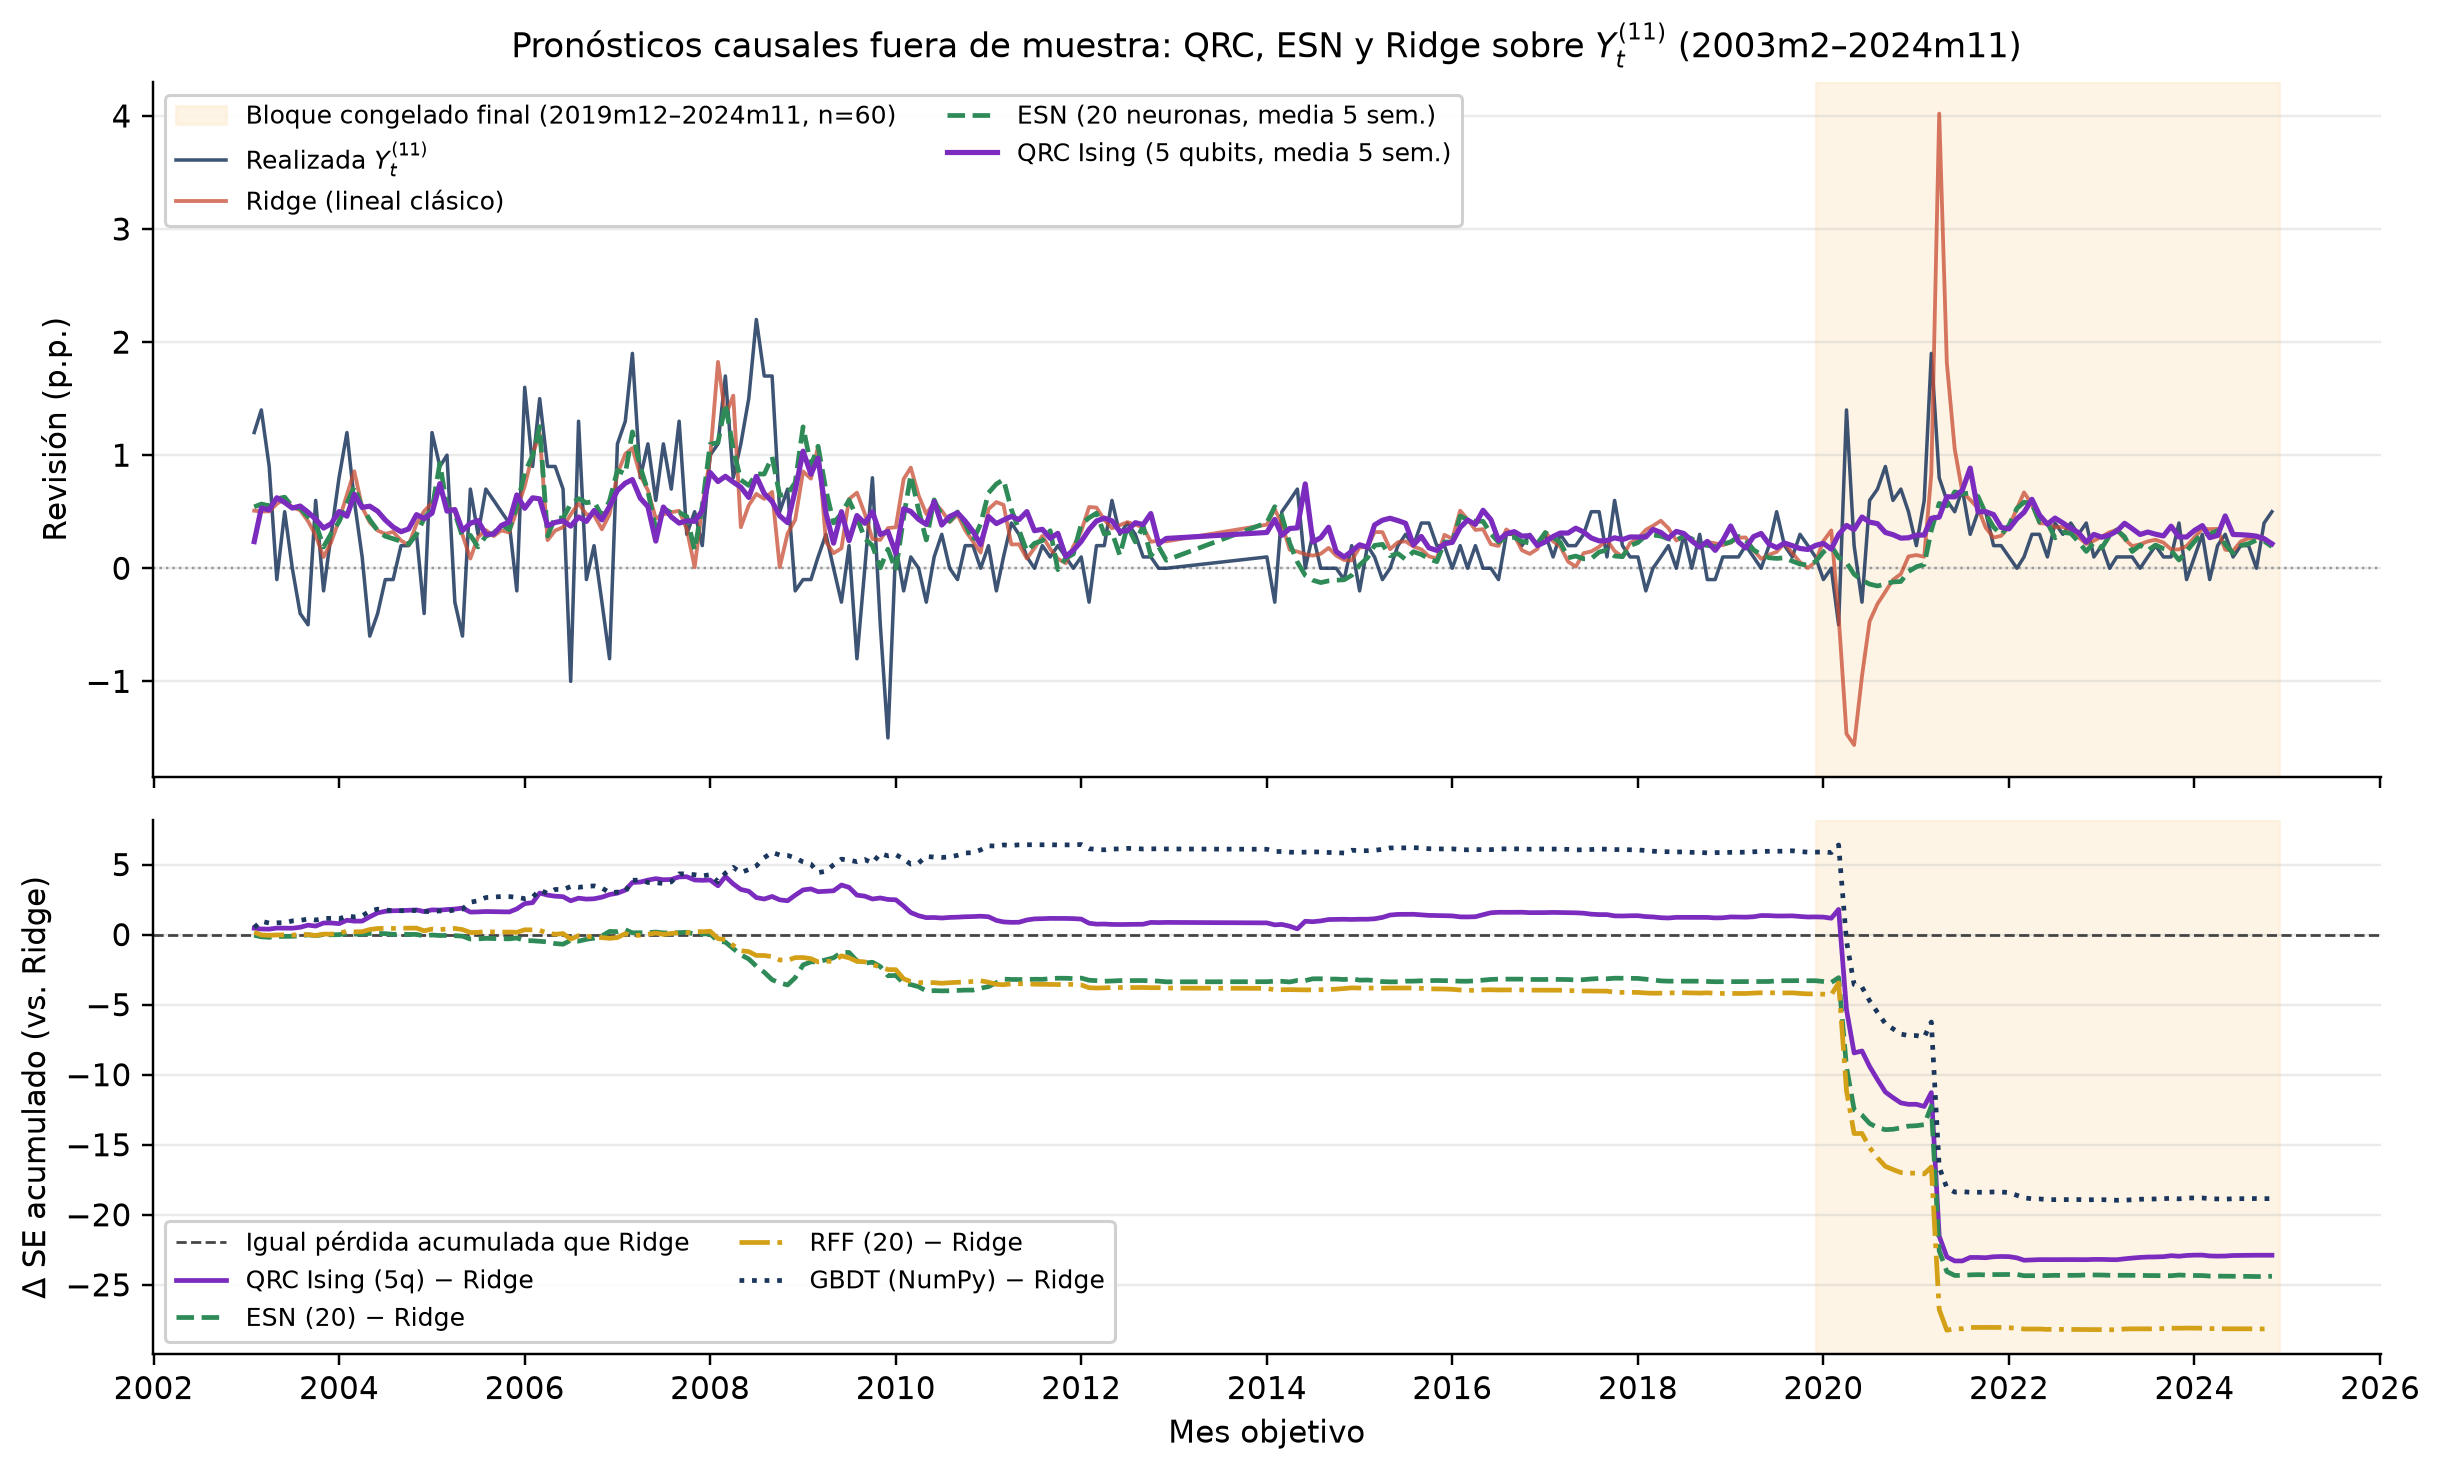
\includegraphics[width=0.95\textwidth]{figuras/etapa4_reservorios_oos.png}
  \apanota{Tomado de \codigo{output/etapa4\_reservorios/etapa4\_reservorios\_oos.png}. La caída de pérdida acumulada en 2020--2021 muestra el ahorro de error frente a la extrapolación lineal.}
\end{figure}

\begin{figure}[htbp]
  \caption{Estabilidad por regímenes y dispersión Monte Carlo entre cinco semillas (Etapa~4)}
  \label{fig:etapa4_estabilidad}
  \centering
  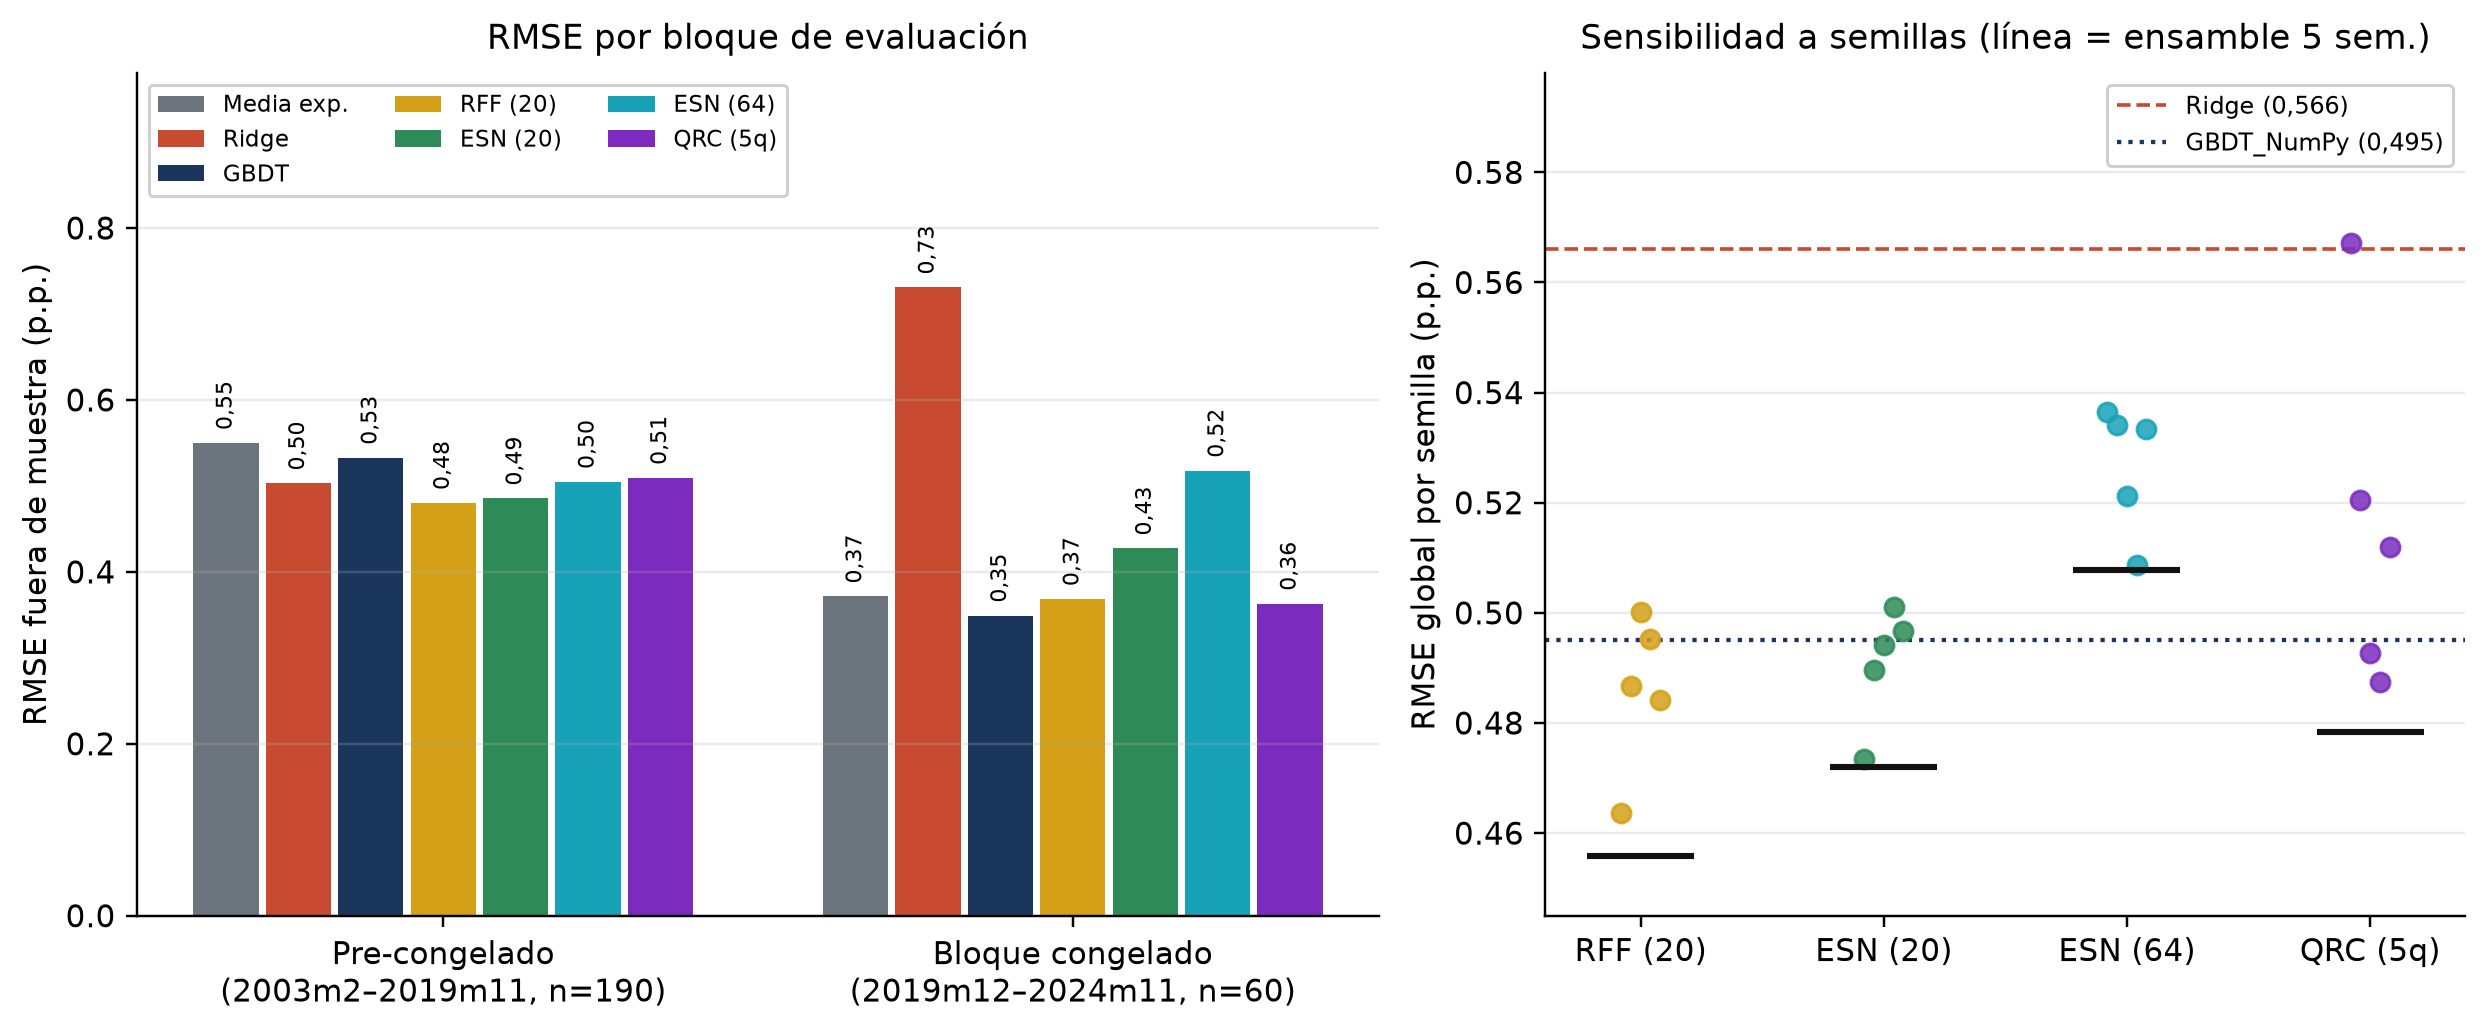
\includegraphics[width=0.95\textwidth]{figuras/etapa4_estabilidad_regimenes.png}
  \apanota{Tomado de \codigo{output/etapa4\_reservorios/etapa4\_estabilidad\_regimenes.png}. Se distingue cómo el promedio de cinco semillas mejora el RMSE individual en todas las arquitecturas.}
\end{figure}

\apabibliografia

\end{document}
